\chapter{Analisis}
\label{chap:analsa}

\section{Kondisi IDE UNPAR}
\label{sec:Kondisi IDE UNPAR} 
IDE UNPAR sudah mengalami perubahan dan penyesuaian agar dapat digunakan, perubahan dan penyesuaian tersebut yang harus diterapkan juga didalam Moodle mobile. Perubahan dan penyesuain yang dimaksud adalah perbedaan dari tampilan dan fitur IDE UNPAR yang tidak ada dalam situs Moodle standar dan dapat dilihat oleh peneliti. Perubahan dan penyesuaian  terhadap IDE UNPAR adalah : \cite{IDEUNPAR}

\begin{itemize}
\item Penggunaan tema Snap Moodle. perubahan ini terlihat ketika memeriksa elemen dari IDE UNPAR pada baigan HTML \textit{tag}.
\item Mata kuliah dan peserta mata kuliah.
\item \textit{Banner} pada halaman utama.
\item Bagian panduan digital.
\item Video YouTube tersemat.
\item Branding UNPAR
\item SSO
\end{itemize}

Perubahan dan penyesuaian diatas tidak semua dapat diterapkan ke dalam Moodle mobile. Penggunaan tema Snap dapat dilakukan dikarenakan Moodle mobile sudah tidak lagi mengukung penggunaan tema. Sehingga tampilan pada Moodle mobile akan diubah dengan mengubah \textit{source code}. \textit{Banner} pada halaman utama, bagian panduan digital dan branding UNPAR juga akan dilakukan dengan mengubah \textit{source code}, karena pada situs IDE UNPAR perubahan dan penyesuaian tersebut dilakukan pada tema yang digunakan. SSO juga tidak akan digunakan karena peneliti tidak memiliki akses SSO UNPAR.

Moodle mobile memungkinkan untuk mengatur \textit{URL preset} agar saat Moodle mobile dijalnkan, akan langsung diahlikan ke \textit{URL} tersebut. Namun ketika \textit{URL} IDE UNPAR digunakan terdapat \textit{error} dimana variable \texttt{\$urlscheme} memiliki nilai variable yang sudah diubah, dimana seharusnya variable tersebut berisi \texttt{moodlemobile://token=...} melainkan berisi \texttt{ide.unpar.ac.id://token=....}. Mengubah variable \texttt{urlscheme} pada Moodle mobile tetap tidak memungkinkan  IDE UNPAR diakses melalui Moodle mobile. Karena  adanya konfigurasi yang tidak dapat diakses untuk menghubungkan IDE UNPAR maka situs demo akan digunakan.
%tidak dapat digunakannya akses ke IDE UNPAR maka penilitian ini akan menggunakan sebuah situs demo yang dibuat dengan Moodle atau Moodle demo.

\section{Moodle demo}

Moodle demo dengan \textit{URL} \url{https://moodledemo.pascal.id} adalah situs demo yang akan digunakan. Moodle demo akan berfungsi sebagai \textit{web service} yang diakses oleh Moodle mobile. Sehingga Moodle demo akan menyimpan data mahasiswa, dosen, mata kuliah dan \textit{plugin} yang  ada pada IDE UNPAR untuk digunakan di dalam Moodle mobile. 
\subsection{Mata kuliah dan peserta mata kuliah}

Data yang berada pada Moodle demo berasal dari mata kuliah yang ada di IDE UNPAR diberikan oleh pembimbing, sehingga pada data mata kuliah tersebut terdapat bahan dan tugas. Peserta dari mata kuliah tersebut dibuat dengan sendiri mengikuti format penamaan yang berada di IDE UNPAR dan ada tiga peserta yang diikutkan dalam mata kuliah tersebut dengan tiga role yang berbeda yaitu \textit{teacher} yang dianggap seabagai dosen, \textit{non-editing teacher} dianggap sebagai asisten dosen dan \textit{student} dianggap sebagai mahasiswa.

\subsection{\textit{Plugin} dan tema}

\textit{Plugin} yang digunakan oleh Moodle demo adalah plugin standar Moodle karena pada IDE UNPAR tidak ditemukannya \textit{plugin} tambahan selain tema yang digunakan. \textit{Plugin} tema tidak harus digunakan karena tidak mempengaruhi Moodle mobile, namun dengan tujuan mengimitasi IDE UNPAR tema akan tetap digunakan karena peletakan \textit{banner}, video YouTube tersemat dan bagian panduan digital bergantung pada tema yang digunakan oleh IDE UNPAR. Tema pada situs moodle dapat dipasang dengan memasukkan file tema yang diambil dari situs \url{https://moodle.org/plugins/} ke dalam folder \texttt{/moodle/theme}. Setelah file berada dalam folder tersebut maka pada situs Moodle dibagian \textit{themes} akan muncul opsi tema yang baru saja dimasukkan.

Korsel pada untuk Moodle demo dapat dipasang dengan mengakses halaman menu tema. Pada halaman tersebut pilih opsi \textit{Cover display}, dalam opsi tersebut akan ada bagian untuk mengaktifkan dan memasang korsel untuk situs Moodle. Jumlah maksimal koresel yang dapat dipasang adalah 3 korsel. Korsel pada moodle demo ini bertujuan untuk mengimitasi \textit{banner} yang berada pada IDE UNPAR.

Bagian panduan digital pada IDE UNPAR adalah bagian \textit{featured course} yang diubah judulnya menjadi "panduan digital". Menggunakan fitur ini pada Moodle demo dapat dilakukan dengan mengakses halaman menu tema seperti pada Gambar \ref{fig:featured courses}, dan memilih opsi \textit{featured course} pada halaman tersebut. Jumlah \textit{course} maksimal yang dapat ditampilkan adalah 8. Karena peniliti tidak memiliki akses untuk \textit{course} panduan digital IDE, maka \textit{course} yang ditampilkan adalah \textit{course} yang sudah dimasukkan. Perubahan yang terjadi disini tidak akan terimplementasi dalam Moodle mobile.

\begin{figure}[H] 
	\centering  
	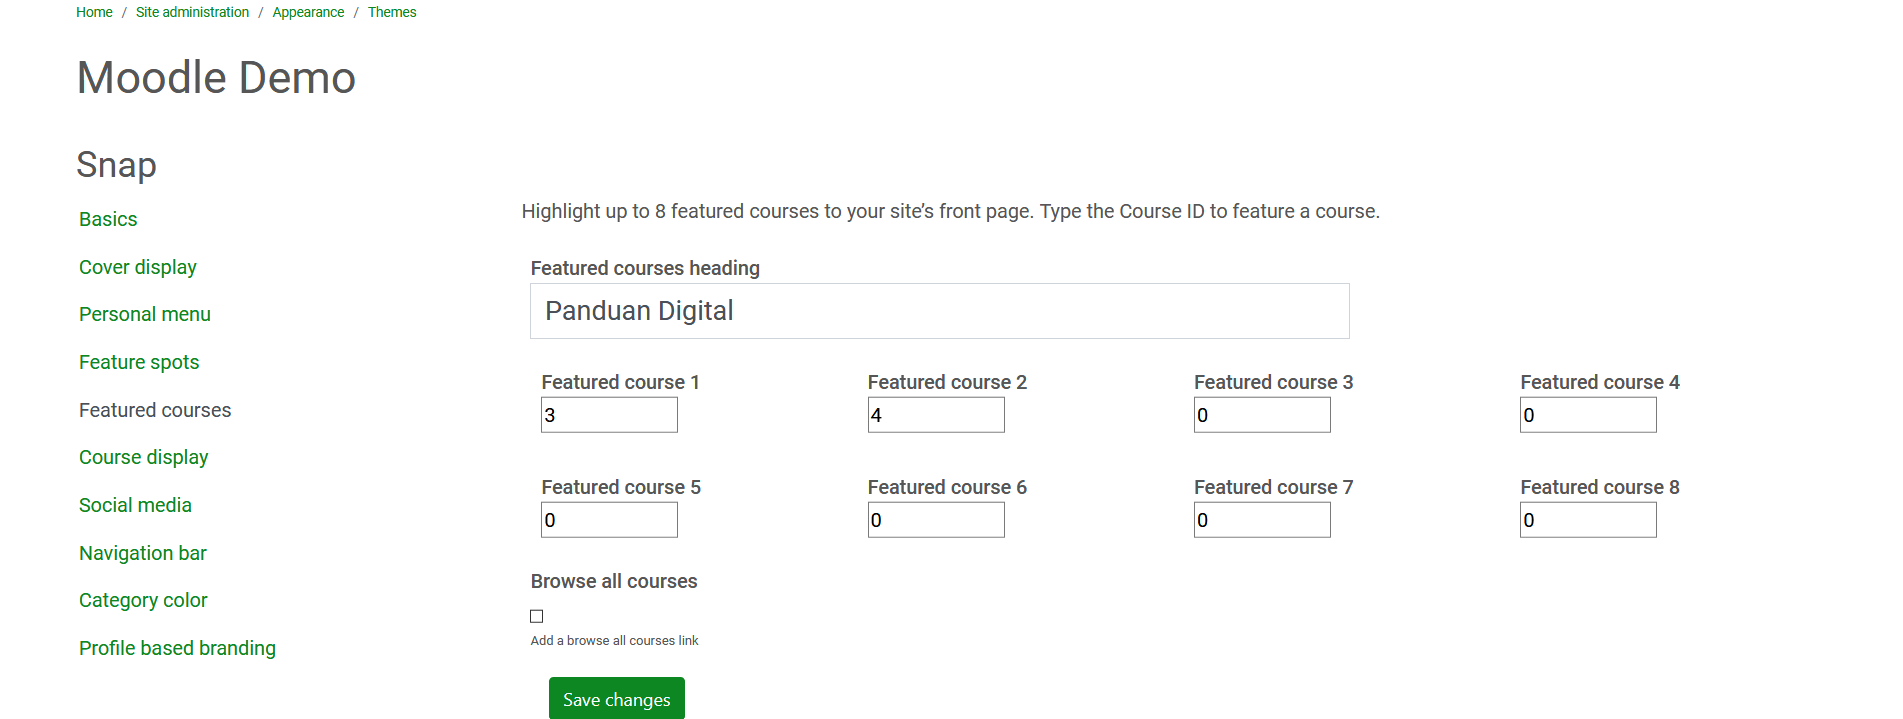
\includegraphics[scale=0.16]{featured-courses.png}  
	\caption[Halaman \textit{Featured Courses}] {Halaman \textit{Featured Courses}} 
	\label{fig:featured courses} 
\end{figure} 


Menambahkan sematan video YouTube dapat dikaukan dengan menekan tombol ikon roda gigi, kemudian memilih opsi \textit{turn editing on}. Dalam mode pengeditan tekan ikon kertas dan pensil seperti pada Gambar \ref{fig:editingmode}. Pada halaman edit, masukkan tag \textit{iframe} HTML dengan link video untuk menyematkannya. Seluruh perubahan yang dilakukan dalam mode pengeditan Moodle demo akan langsung terimplementasi juga pada Moodle mobile dalam halaman yang sesuai.

\begin{figure}[H] 
	\centering  
	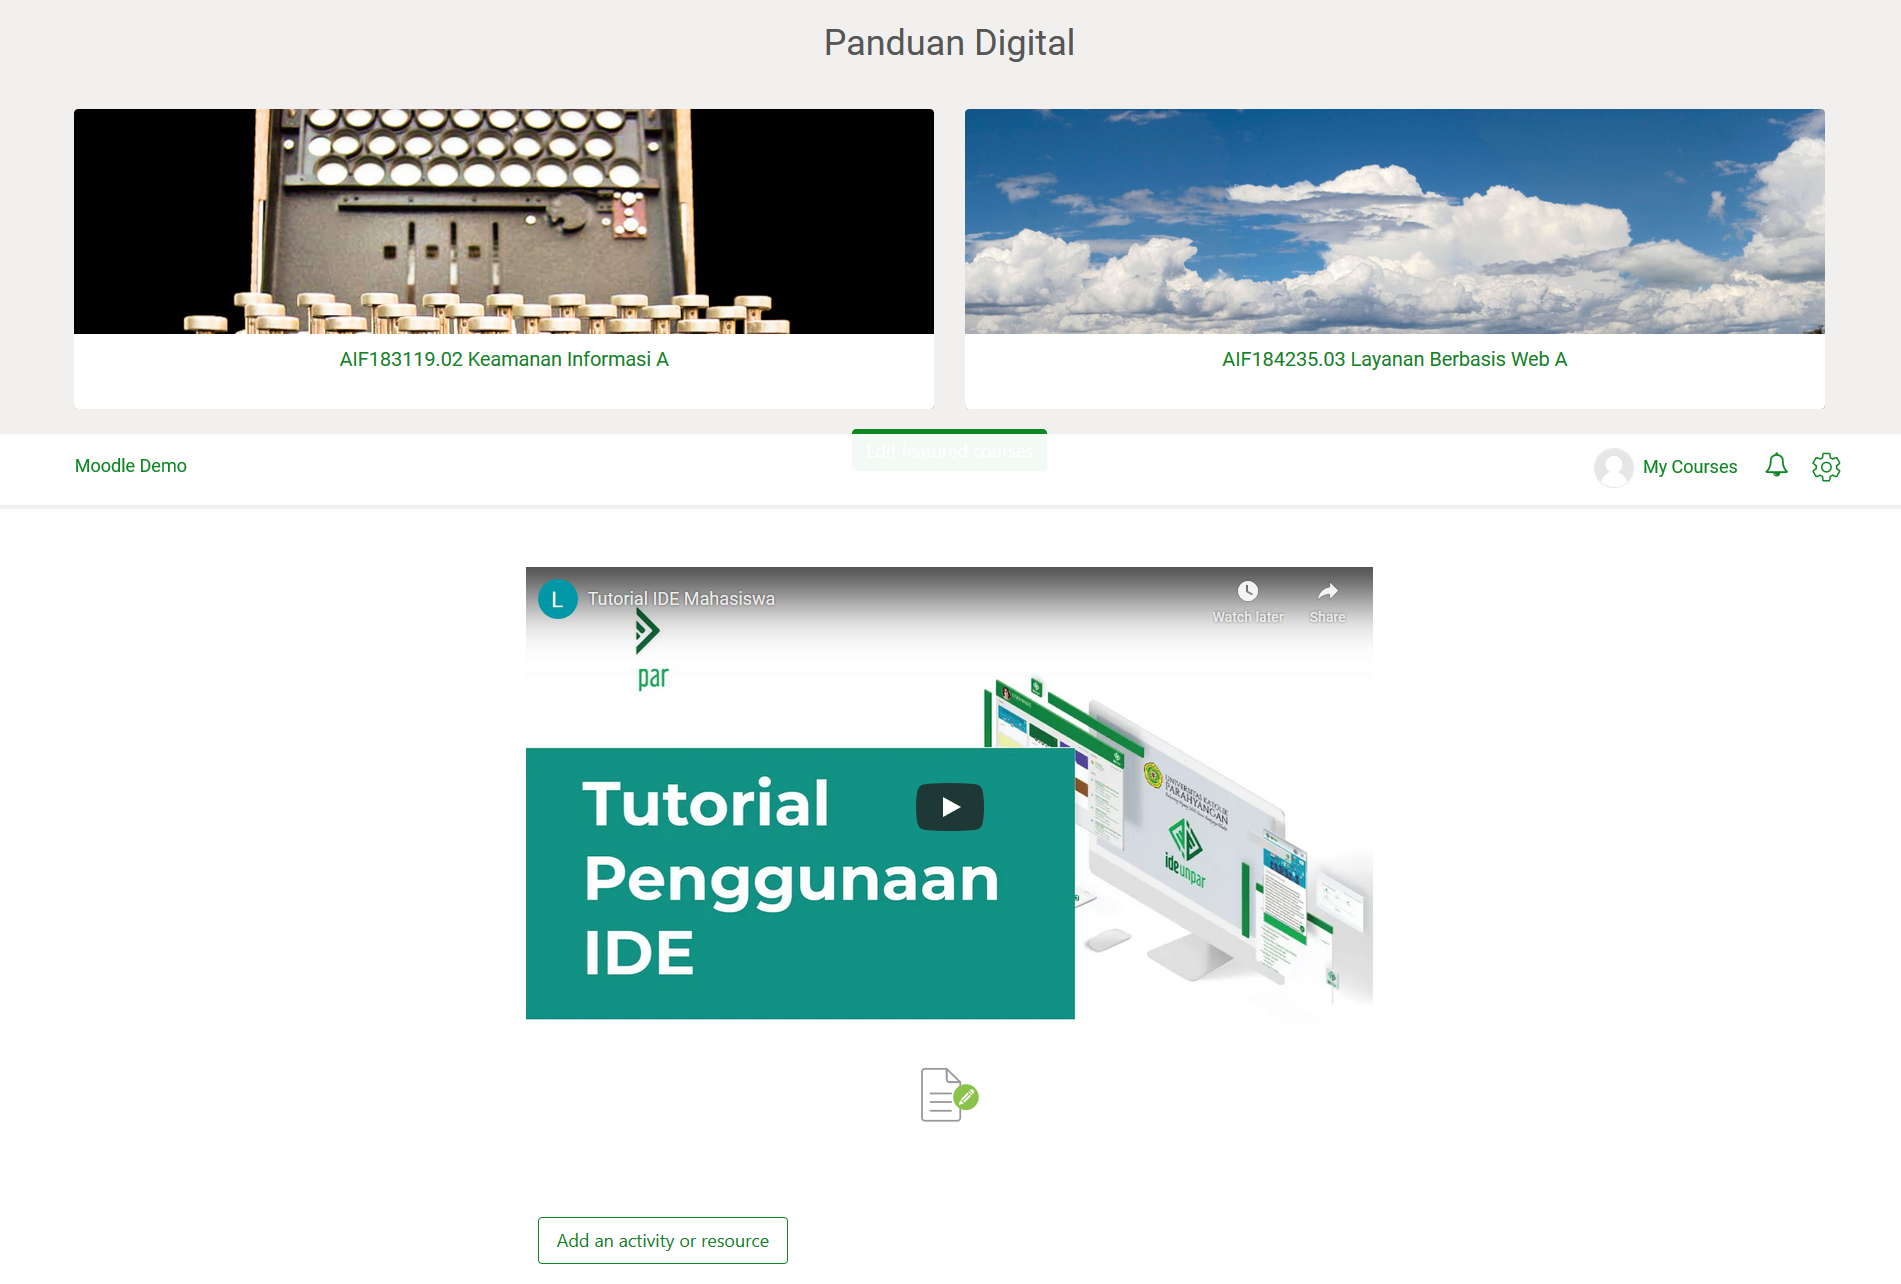
\includegraphics[scale=0.16]{demo-edit-mode.png}  
	\caption[Mode pengeditan] {Mode pengeditan} 
	\label{fig:editingmode} 
\end{figure} 

\section{Lisensi Moodel mobile}

Moodle mobile dilisensikan dengan lisensi \textit{Apache 2.0}\cite{Moodlemobile:license}. Lisensi tersebut mengizinkan untuk melakukan reproduksi dari Moodle mobile dengan atau tanpa modifikasi. Seperti yang disebut pada poin 4 lisesnsi dengan judul \textit{"Redistribution"}, hal-hal tersebut dapat dilakukan apabila memenuhi syarat-syarat yang tertera. Syarat-syarat yang dimaksud adalah :
\begin{itemize}
\item Aplikasi yang dibuat harus disertakan dengan salinan lisensi \textit{Apcahe 2.0}.
\item Seluruh file yang dimodifikasi harus menyertakan pemberitahuan yang jelas bahwa file tersebut sudah dimodifikasi.
\item Seluruh paten, \textit{trademark}, \textit{copyright} dan pemberitahuan atribusi harus disimpan dalam bentuk sumber untuk seluruh aplikasi yang akan didistrubusikan.
\item Apabila aplikasi sumber menyertakan file teks dengan judul \textit{\textbf{NOTICES}}, maka selurh aplikasi yang akan didistribusikan harus menyertakan salinan yang dapat dibaca.
\end{itemize}
Gagal memenuhi syarat-syarat di atas akan mengakibatkan lisensi untuk aplikasi yang telah dimodifikasi dan didistribusikan berrsifat tidak sah.